\chapter{Physics Background} \label{ch:physBKGD}
%\newpage
\section{Introduction}
Introduction about the chapter.

\section {Standard Model of Particle Physics} \label{sec:stdModel}

CERN\footnote{European Organization for Nuclear Research}

\begin{figure}[htbp!]
\begin{center}
  \includegraphics[width=1.0\textwidth]%
%    {figures/instrument/25ns_fill_scheme.png}% picture filename
%  {figures/model/Standard_Model_of_Elementary_Particles.svg.png}
  {figures/intro/discoveries.pdf}
	\captionsetup{format=hang}

  \caption{The discoveries of fundamental particles of the Standard Model vs time \cite{Thesis:Tuna}}
\end{center}

\end{figure}


\subsection {Elementary Particles}

\subsection {Fundamental Forces}




\begin{figure}[htbp!]
\begin{center}
  \includegraphics[width=0.7\textwidth]%
%    {figures/instrument/25ns_fill_scheme.png}% picture filename
%  {figures/model/Standard_Model_of_Elementary_Particles.svg.png}
  {figures/intro/Standard_Model_of_Elementary_Particles.svg_wiki}
	\captionsetup{format=hang}

  \caption{The Standard Model of Elementary Particle Physics with three generations
of matter fermions, gauge bosons and a Higgs boson. Figure taken from \cite{wiki:Figure}}
\end{center}

\end{figure}


\begin{table}
\begin{center}
    \begin{tabular}{| l | l | l | l |}
    \hline
    {\bf Interaction} & {\bf Strength} & {\bf Theory} & {\bf Mediator} \\ \hline
    Strong & 10 & Quantum Chromodynamics & Gluon \\ \hline
    Electromagnetic & $10^{-2}$ & Quantum Electrodynamics & Photon \\ \hline
    Weak & $10^{-3}$ & Flavordynamics &  W and Z Bosons\\ \hline
    Gravitation & $10^{-42}$ & Geometrodynamics & Graviton \\
    \hline
    \end{tabular}
     \caption{Rough order of the interaction strengths, the mediator and the theory, which describes
these interactions}

\end{center}
\end{table}


\section{Luminosity}
%\subsection{Introduction}

The quantity that measures the ability of a particle collider to produce the required number of interactions is called the luminosity $\mathcal{L}$. Its precise knowledge is important since for many cross-sections measurements the uncertainty factor on the luminosity dominates the final result. Luminosity is the proportionality factor between the number of events per second $R(t)$ at a given time $t$ and its production cross-section $\sigma_{P}$ for a process:

\begin{equation} \label{eq:rate}
R(t) = \mathcal{L}(t) \cdot \sigma_{P}
\end{equation}

This defines the so-called instantaneous luminosity commenly measured in units of $cm{-2} s^{-1}$. Typically running conditions vary with time $t$. Therefore, the luminosity of a collider also has a time dependence that needs to be carefully measured to arrive at an (time) integrated luminosity for a given data taking period which is given as:

\begin{equation} \label{eq:instLumi}
\mathcal{L}_{int} = \int \mathcal{L}(t) dt
\end{equation}
and measured in units of $b^{-1}$. The delivered integrated luminosity, which refers to the integrated luminosity which the machine has delivered to an experiment, and recorded integrated luminosity, which refers to the amount of data that has actually been stored to disk by the experiments typically differ and hence an independent measurement by experiment is necessary.

As $\mathcal{L}$ is process-independent it is possible to measure the luminosity with any process whose cross-section is known. For a precise luminosity determination, however, it is essential that the process has precise theoretical predictions and at the same time that its rate can be accurately measured, i.e. enough are produced in a limited time interval. The production of $Z^{0}$ bosons $(pp \rightarrow Z^{0} X) $ that decay into leptons, particularly muons $(Z^{0} \rightarrow \mu^{+} \mu^{-})$, is such a "standard candle process", because the leptons can be well identified and theoretical prediction of the cross section has only a few percent relative uncertainty. The cross-section of $Z^{0}$ production is large enough and there are almost no fake signals.


% Colliding Beams
\begin{figure}
\centering
\begin{tikzpicture}[scale=1.25]
%    \draw [red] (0,0) ellipse (2cm and 0.25cm);
    \draw [->, red] (-1,0.5) -- (1,0.5);
    \node (draw) at (0,1) {$N_{1} \rho_{1}(x,y,s;-s_{0})$};
%  \node [cylinder, gray!50, rotate=0, draw,
  \node [cylinder, red, rotate=0, draw,
    minimum height=3cm, minimum width=1cm] at (0,0) {};

    \filldraw (2.5,0) circle (1pt);

  \node [cylinder, blue, rotate=180, draw,
    minimum height=3cm, minimum width=1cm] at (5,0) {};

    \draw [->, blue] (6,0.5) -- (4,0.5);
    \node (draw) at (5,1) {$N_{2} \rho_{2}(x,y,s;s_{0})$};

    \draw[->] (-4,0) -- (8,0) node[right] {$z$};


\node[align=center] at (2.5,-1) (ori) {$A_{eff}$};
\draw [->] (2.5,-0.9) --(1.1,0);

\end{tikzpicture}
\caption{Colliding beam bunches} \label{fig:collBeams}
\end{figure}


The instantaneous luminosity can be extracted from certain beam parameters. A simplified case for a head-on collision of two bunches is shown in Figure \ref{fig:collBeams}. The luminosity can be expressed from geometry and the number of particles in each of the two colliding beam bunches $n_{1(2)}$:

\begin{equation} \label{eq:intLumi}
\mathcal{L} = \frac{n_{1} n_{2} f}{A_{eff}}
\end{equation}

\noindent
with f the collision frequency. Beam parameters for the LHC are listed in Table \ref{tbl:beamParam}. Of the possible 3564 bunches only $n_{b} = 2808$ are filled reducing the peak luminosity accordingly. The beam current $I_{1(2)}$ is given in terms of the charge of the beam particle $e$ and the collision frequency f as $I_{i} = e_{i} f n_{i}$. Hence, one obtains

\begin{equation}
\mathcal{L}_{int} = \frac{I_{1} I_{2}}{e^{2} f A_{eff}}
\end{equation}

\begin{figure}
\begin{center}
  \includegraphics[width=1.0\textwidth]%
  {figures/intro/crosssections.pdf}
	\captionsetup{format=hang}
  \caption{The cross sections and expected production rates at the LHC and the Tevatron.}
  \label{fig:crossSection}
\end{center}

\end{figure}


With a nominal instantaneous luminosity of $\mathcal{L} = 10^{34} cm^{-2} s^{-1} (= 10 nb^{-1} s^{-1})$ and a Higgs production cross section of $\sigma \simeq 0.1 nb$ one expects about 1 Higgs per second. Figure \ref{fig:crossSection} shows the cross sections for several processes at a 10 times lower  nominal luminosity that has been achieved so far with the LHC. At this luminosity also about 100 $Z^{0}$ particles are produced per second. Only 3.4 \% of $Z^{0}$'s decay into a muon pair resulting in about 3 $Z^{0}$ particles per second that are potentially detected with CMS.


\begin{table}[htp]
\begin{center}
\begin{tabular}{|l|c|c|}
\hline
{\bf Beam Parameter} & {\bf Unit} & {\bf Value} \\ \hline
Proton Energy & [GeV] & 6500 \\ \hline
Stored energy per beam & [MJ] & 363 \\ \hline
Number of particles per bunch $n_{i}$ & & $1.15 \times 10^{11}$ \\ \hline
Number of bunches $n_{b}$ & & 2808 \\ \hline
Bunch collision frequency $f$ & MHz & 40 \\ \hline
Circulating beam current & [A] & 0.584 \\ \hline
Transverse beam size ($\sigma_{x,y}$) & $\mu m$ & 16.7 \\ \hline
RMS bunch length ($\sigma_{z}$ & cm & 7.55 \\ \hline
Geometric luminosity reduction factor F & & 0.836 \\ \hline
Peak luminosity in IP1 and IP5 & [$cm^{-2} sec^{-1}$] & $10^{34}$ \\ \hline \hline

\end{tabular}
\end{center}
    \captionsetup{format=hang}
     \caption{LHC beam parameters relevant for the peak luminosity \cite{fill-schemes}}
    \label{tbl:beamParam}
\end{table}%


Assuming that the transverse profile of the two bunches distribute identically and that the profiles do not change along the bunch a good approximation is a Gaussian profile for the beam transverse distribution in $x$ and $y$, each characterized with a standard deviation $\sigma_{x}$ and $\sigma_{y}$, respectively. In this case $A_{eff} = 4 \pi \sigma_{x} \sigma_{y}$. It implies that the profiles in $x$ and $y$ are not correlated.


The two beams at the LHC corss each other under an angle of $\theta_{C} = 285 \mu rad$ to direct the beams after collision into their respective vacuum pipe and to avoid multiple unwanted interactions. Figure \ref{fig:rotBeams} shows a schematic illustration of the beam crossing. It also shows a change in the profile along the beam width. The correct evaluation of the effective beam size is obtained from an overlap integral of beam density distribution functions in all three coordinates \cite{lumiConcepts}. For small angles, Gaussian profiles and $\sigma_{x} \simeq \sigma_{y}$ in good approximation this results in the so called geometric luminosity reduction factor F, given as


\begin{equation} \label{eq:lumiAcc}
F = \left(  \sqrt{1 + \left( \frac{\theta_{c} \sigma_{z}}{2 \sigma^{*}} \right ) ^{2}}  \right) ^{-1}
\end{equation}

that multiplies eq. \ref{eq:intLumi}.

% Colliding Beams at some angle

\begin{figure}[h]
\centering
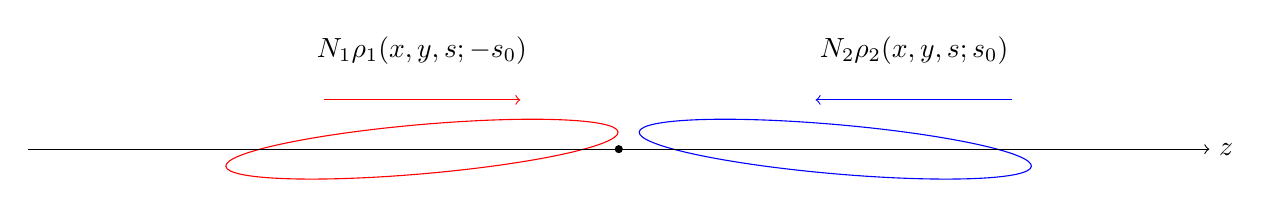
\begin{tikzpicture}[scale=1.25]
    \draw [red,rotate around={5:(0,0)}] (0,0) ellipse (2cm and 0.25cm);
    \draw [->, red] (-1,0.5) -- (1,0.5);
    \node (draw) at (0,1) {$N_{1} \rho_{1}(x,y,s;-s_{0})$};

   \filldraw (2,0) circle (1pt);

    \draw [blue,rotate around={-5:(4.2,0)}] (4.2,0) ellipse (2cm and 0.25cm);
    \draw [->, blue] (6,0.5) -- (4,0.5);
    \node (draw) at (5,1) {$N_{2} \rho_{2}(x,y,s;s_{0})$};

%    \draw [->] (-4,0) -- (0,0) -- (1,0) -- (8,0);
    \draw[->] (-4,0) -- (8,0) node[right] {$z$};

\end{tikzpicture}
\caption{Beams colliding at some angle} \label{fig:rotBeams}
\end{figure}


In practice, however, there are complications: beams do not factorize as the profile changes over the length of the bunch and bunches do not collide exactly head-on but with offsets. Imperfections in the beam steering lead to widening of the beam profile and in turn smaller luminosity. So far also a uniform population of the beam bunches is assumed while in reality the actual fill pattern can vary. The LHC provides measurements of beam currents and beam profiles along the LHC accelerator but not in the vicinity of the interaction points. Furthermore, the beam parameters and conditions change over the time period of a LHC fill. To arrive at the best time-integrated luminosity the time integral has to be taken over time intervals short enough to measure significant variations and exclude dead times. Typically the beam intensity decays exponentially with time resulting in a similar reduction in the instantaneous luminosity. The effective mean lifetime of the luminosity is further reduced by the increase of the transverse and longitudinal beam size over time. To reduce uncertainties due to extrapolation from beam parameter measurements the CMS experiment has to measure the relative luminosity with dedicated detectors and calibrate them with standard candle processes or dedicated calibration runs of the LHC. Figure \ref{fig:lumiCompare} shows a comparison of the luminosity measurement via LHC parameters and Pixel Luminosity Detector for the CMS experiment.



\begin{figure}[htbp!]
\begin{center}
  \includegraphics[width=1.0\textwidth]%
%    {figures/instrument/25ns_fill_scheme.png}% picture filename
%  {figures/model/Standard_Model_of_Elementary_Particles.svg.png}
  {figures/lumi/Fill5253LumiCompare.png}
	\captionsetup{format=hang}
  \caption{Comparison of luminosity measured via LHC beam parameters and Pixel Luminosity Detector for the CMS experiment, Fill 5253. Drops signify change in run number.}
  \label{fig:lumiCompare}
\end{center}

\end{figure}
